\section{System Model}\label{sec_system}
The system model is composed of three parts: software applications $A=\{a_1, a_2,...a_{l_c}\}$, an execution platform $p=M=\{m_1, m_2,...m_{l_m}\}\cup B$, and an allocation scheme $f:A\mapsto B$ as illustrated in the Figure \ref{fig_softwareallocation}. The applications are user-defined software systems, such as x-by-wire, electronic throttle control, flight control, etc., which are developed using software components \cite{softwarecomponents}\cite{Crnkovic2002BuildingSystems}. The applications are deployed on a network of computation nodes, which are logical hardware components that provide an execution platform together with operating systems and middleware software applications. The allocation scheme defines the mappings of the software components to computation nodes and  denotes the deployment of the software applications.

\begin{figure}[!h]
\centering
\includegraphics[scale=0.6]{}
\caption{System Model.}
\label{fig_softwareallocation}
\end{figure}

The system realizes fault-tolerance by replicating two or more software components on distinct nodes in order to meet reliability requirements. Furthermore, the system is real time, that is applications must exhibit functional behavior on timely manner. Essentially, the applications are annotated with timing information both at the higher-level (user-level) abstraction and lower-level (or operating system level), respectively via action-reaction (or stimuli-response) timing constraints and timing models of operating system processes (or tasks). The allocation scheme should satisfy the reliability and timing requirements of the applications. Since, different allocation schemes provide different system performance, we consider optimizing of the design on the basis of power consumption at the same time fulfilling the stated reliability and timing requirements of the applications.


\paragraph{Notations}  For the purpose of smooth reading, we use the following mathematical notations to describe the system model, define the software allocation problem, explain and analyze the problem throughout the paper. %For convenience, we use similar symbols intermittently, in which case their usage is explained in the context and the latter overrides the respective notation.
\begin{table}[]
\begin{tabular}{@{}llp{0.65\textwidth}@{}}
\toprule
 & Notation                        & Description                                                               \\ 
\midrule
$\bullet$ & $C=\{c_i\ |i\in[1,I]\}$         & a set of software components, where $I$ is caridnatlity of $C$, that is $I=\abs{C}$ \\
$\bullet$ & $c_i^k$                         & the $k^{th}$ replica (or prototype of) the $c_i$ software component, and $K=\abs{replica(c_i)}$\\
$\bullet$ & $R=\{r_i\ |i\in[1,N]\}$         & a set of runnables, where $N=\abs{R}$                                 \\
$\bullet$ & $M=\{m_i\ |i\in[1,J]\}$         & a set of computation nodes (or ECUs), $J=\abs{M}$                      \\
$\bullet$ & $(V,E)$                       & a software application, modeled as a digraph of runnable nodes $V$ and edges $E$             \\
$\bullet$ & $\Gamma=\{\Gamma_i\ |i\in[1,M]\}$ & a set of end-to-end paths (or cause-effect chains) of the graph $a$                      \\
$\bullet$ & $\Gamma_i=(V_{r_i})_{i=1}^Z$   & a chain of runnable nodes, where $Z=\abs{\Gamma_i}$ is the length of the chain           \\ 
$\bullet$ & $\zeta:\Gamma_i\mapsto \Gamma_i^T$ & a function that groups and maps runnables to operating system tasks, $T=\{\tau_i\ |i\in[1,H]\}$, where $H=\abs{T}$   \\
$\bullet$ & $P$                            & power consumption of a software application                                             \\
\bottomrule
\end{tabular}
\end{table}

%he system overview is illustrated illustrated in Figure \ref{fig_softwareallocation}.
%on the computation nodes (or mappings of the software components) which is a network of heterogeneous nodes with possibly different processor frequencies, power consumption, and failure-rates. The allocation scheme, which defines a mapping relation from software components to computational nodes, guarantees that the extra-functional properties such as application reliability and timing requirements are met. Furthermore, it takes the optimization of power consumption as its objective in the allocation process.

\subsection{AUTOSAR System Model}
In this work, we target AUTOSAR-based systems due to the increasing popularity of the standard in  the automotive industry, and the challenges and opportunities that automotive industry is facing especially in resource optimization and dependability of automotive systems. The model is illustrated in Figure \ref{fig_softwareallocation}. Note that our approach can also be applied on different domains of distributed embedded systems with a slight change in the application modeling.
\begin{figure}[!h]
\centering
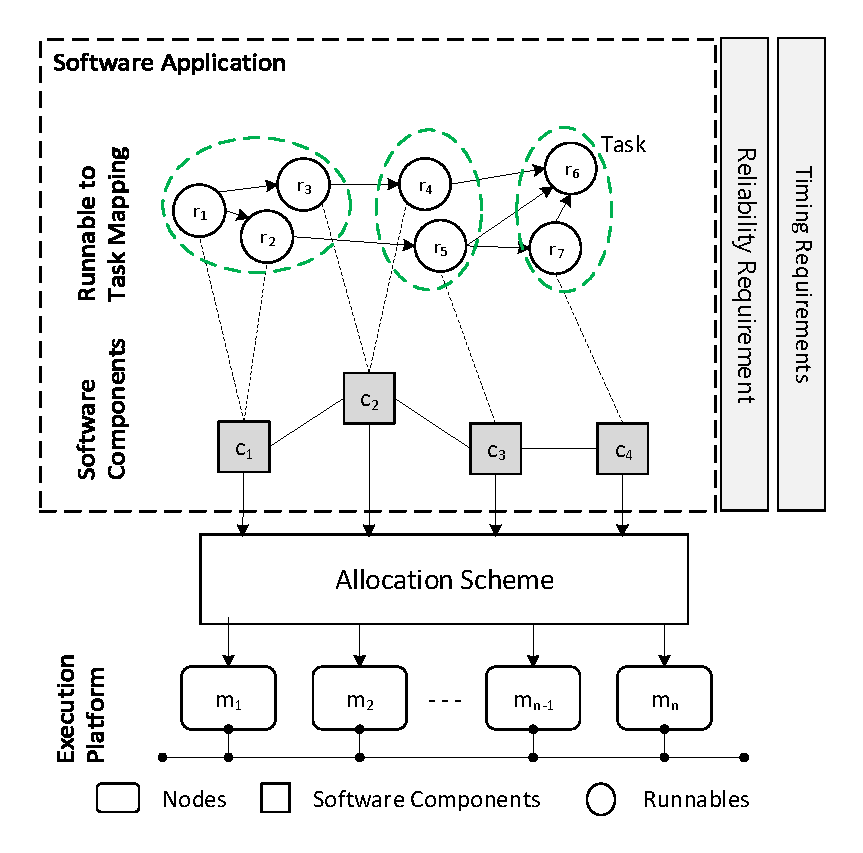
\includegraphics[scale=0.6]{softwareallocation}
\caption{System Model.}
\label{fig_softwareallocation}
\end{figure}

\subsection{Software Application Model}
AUTOSAR software applications are constructed from communicating AUTOSAR application components $\bigcup_{i=1}^{I} C_i$, where the component $c_i^k$ is the $k^{th}$ replica of the component type $C_i$ and $I$ is the number of software component types (or the cardinality of the infinitary union). Each software component co-hosts a set of runnables $R^*\subseteq R$ that are disjoint.

\begin{definition}[AUTOSAR Software Application] For simplicity, we model an AUTOSAR software application $\zeta$ as a \textit{DAG} (directed acyclic graph) $\langle V_r, E\rangle$ of runnable nodes $V_r$, where $\langle u,v\rangle\in E$ is a set of directed links from $u$ to $v$ which denote the logical data flow of the application, and $u,v\in V_r$. A runnable is a tuple $\langle \bigcup_{j=1}^{J} e_{j} , p \rangle$, where $e_{j}$ is the execution of the runnable on node $m_j$ and $p$ is its periodic activation.
\end{definition}

Before software components are allocated to nodes, the runnables are mapped to tasks according to AUTOSAR development approach \cite{AUTOSAR2017SpecificationSoftware}:
\begin{itemize}
\item Case1: A runnable is mapped to a single task as one-to-one, $r\mapsto \tau$
\item Case2: Runnables that are co-hosted in a software component are mapped to a single task, that is a component is mapped to a task as one-to-one, $R_{c_i^k}\mapsto \tau_i^k$
\item Case3: Runnables from the same software components that proceed one another and have the same activation period are mapped to a single task
For more information, please see the AUTOSAR documentation \cite{AUTOSAR2017SpecificationSoftware}.
\end{itemize}

We assume runnables communicate (or send data messages) at the end of the corresponding tasks' executions. The messages are packed into a single frame if destined to the same node otherwise each runnable communicats across a shared bus via a dedicated message entity, which is schedulable by the CAN bus controller. In essence, the assumed read-exec-write semantics of the runnables lowers the number of schedulable messages entities in the bus by facilitating packing of signals at the expense of restrictive (or less flexible) inter-runnables communication.

Furthermore, we assume fixed and dynamic preemptive scheduling policies, that is each tasks sets allocated to a node must be schedulable according to the choice of the scheduling policy. For convenience, we assume priorities are assigned to tasks according to Rate Monotonic (RM) for the case of fixed scheduling policy, that is a task with a lower period get a higher priority.

\subsection{Fault-tolerant Software Application Model}
Redundancy is the most common way to increase the reliability of an application. It can be implemented according to different schemes, such as hot stand-by, cold stand-by, etc~\cite{Dubrova2013Fault-tolerantDesign}. In this work the details of the redundancy scheme are abstracted away under the following assumptions: i) Hot stand-by redundancy technique is used for the replacement of failed components, which are identical and are allocated on different nodes, ii) software components need to be replicated if the application's reliability requirement is not met without replication, otherwise they are not replicated, iii) the time needed to detect and replace a faulty component is considered negligible and will not be taken into account in the response time analysis of tasks and delay calculation of cause-effect chains, iv) Because of its simplicity, the mechanism for detection and replacement of faulty components will be considered fault-free, and therefore will not be included in the reliability calculations.

We denote the $k^{th}$ replica of a software component $c$ as $c^k$, with $1\le k\leq K$; where $K$ is the maximum number of replicas allowed for each application component.

\subsection{Platform Model}
The application is deployed on a network of heterogeneous computing nodes that are connected via a reliable communication network, the CAN bus. The computation node is specified as a 3-tuple $\langle hz, \lambda, p \rangle$, respectively, refer to the processor frequency, failure-rate and power consumption of a computation node. Due to the heterogeneity assumption of the processors, an application maybe be deployed on nodes with higher processor frequencies, and therefore fewer number of nodes in order to minimize the total power consumption of the system. However, due to the application reliability requirement, the application could be deployed differently, and with more resources. The CAN bus is considered reliable, for instance through redundancy. Therefore, its exclusion from the overall calculation of the system's reliability does not impact our proposed software allocation. %Figure~\ref{fig_softwareallocation} illustrates an overview of an AUTOSAR software application deployment on a set of computational nodes via a software allocation scheme that is discussed in Section~\ref{sec_allocation}.

